\underbar{\textbf{\large Ejercicio 1:}}
\begin{figure}[h]
  \begin{center}
    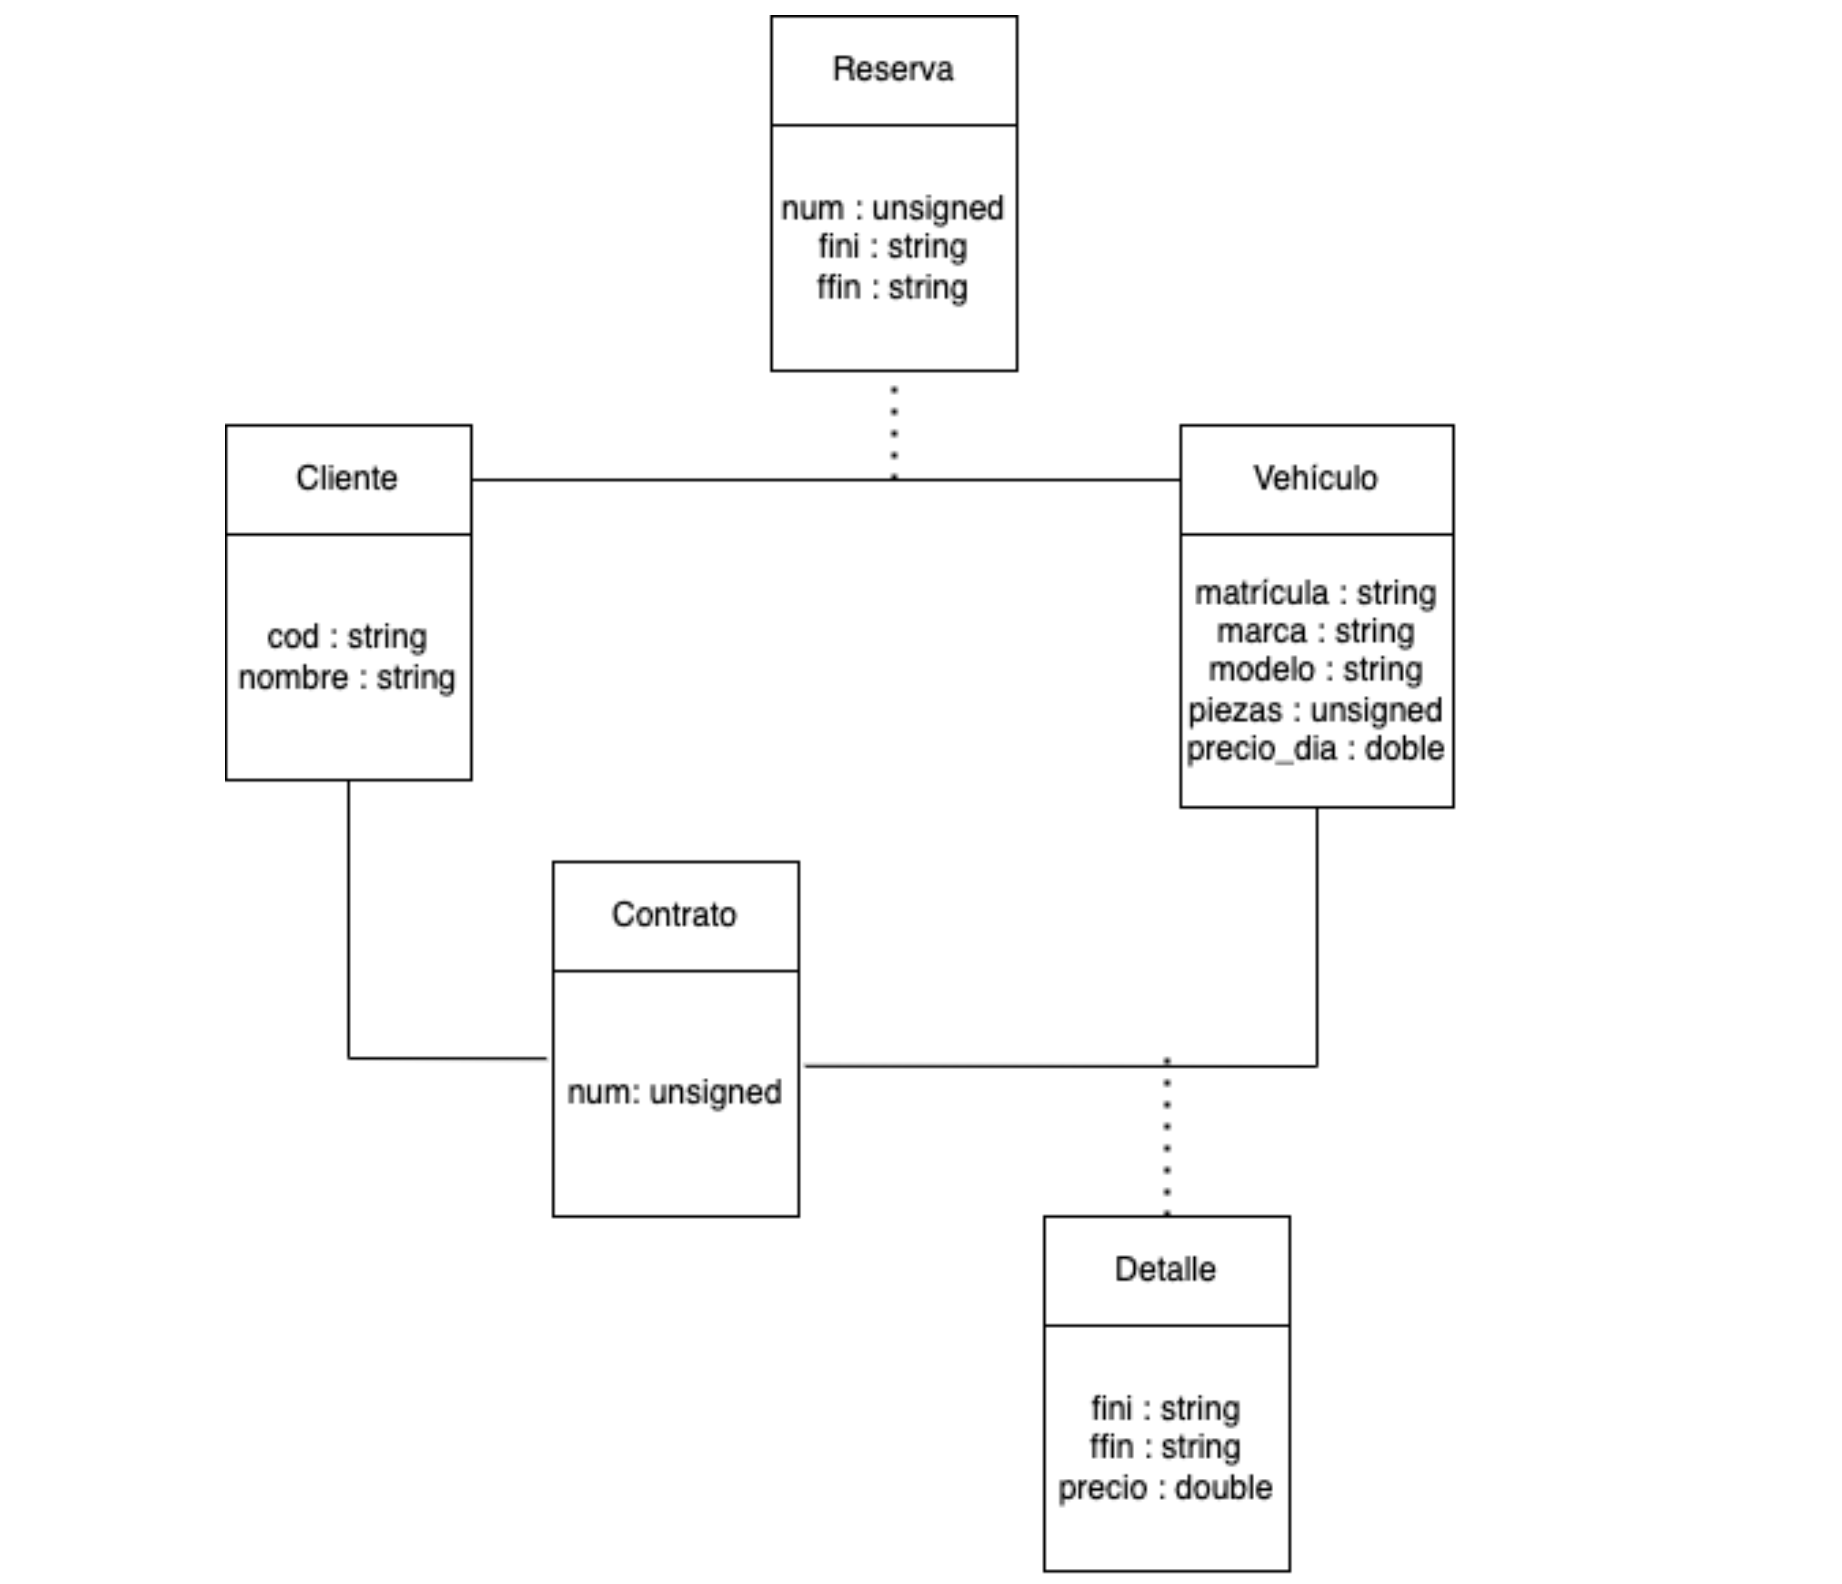
\includegraphics[width=\textwidth]{assets/Junio2022_1.png}
  \end{center}
  \caption{Diagrama de clase del ejercicio}
\end{figure}

Multiplicidad de las relaciones:
Cliente - Vehiculo → N - M; Cliente - Contrato → 1 - N; Contrato - Vehiculo → 1..N - 1..M;
\newpage
\begin{enumerate}[label =\alph*)]
  \item Crea una clase de asociación entre \textbf{Cliente-Vehículo ACV}.

  Implementación de la clase de asociación  \textbf{Cliente-Vehículo ACV}:

  Como vemos es una relación de asignación con una clase de asociación Reserva, como tenemos una multiplicidad N - M pueden haber instancias de cada clase no instanciadas, cosa que tenemos que tener en cuenta los métodos observadores.
\begin{minted}[breaklines]{C++}
class ACV{
  public:
    //Alias de los diccionarios de Cliente y Vehiculo
    typedef std::map<Cliente*,Reserva*> Clientes;
    typedef std::map<Vehiculo*,Reserva*> Vehiculos;
    //Alias de los diccionarios de las relaciones
    typedef std::map<Cliente*,Vehiculos>CVs;
    typedef std::map<Vehiculo*,Clientes>VCs;

    //Método que asocian los objetos
    void setACV(Cliente&,Vehiculo&,Reserva&)noexcept;
    void setACV(Vehiculo&,Cliente&,Reserva&)noexcept;

    //Métodos observadores
    Clientes getClientes(Vehiculo&)const noexcept;
    Vehiculos getVehiculos(Cliente&)const noexcept;
  private:
    CVs directa_;
    VCs inversa_;
};
\end{minted}
Ahora vamos a implementar los métodos (no nos lo pide el enunciado, pero vamos a hacerlo para repasar).
\begin{minted}[breaklines]{C++}
void ACV::setACV(Cliente& c, Vehiculo& v, Reserva& r)noexcept{
  directa_[&c].insert(std::make_pair(&v,&r));
  inversa_[&v].insert(std::make_pair(&c,&r));
}
void ACV::setACV( Vehiculo& v, Cliente& c, Reserva& r)noexcept{
  //delegamos en la operación anterior
  setACV(c,v,r);
}

ACV::Clientes ACV::getClientes(Vehiculo& v)const noexcept{
  //vamos a comprobar si el vehículo está asociado o no
  auto i = inversa_.find(&v);
  //if(i!=inversa_.end())return i->second;
  else{
    //Creamos un conjunto vacio para devolverlo
    ACV::CVs vacio;
    return vacio;
  }
}


ACV::Vehiculos ACV::getVehiculos(Cliente& c)const noexcept{
  //comprobamos que el objeto c Cliente está relacionado
  auto i = directa_.find(&c);
  if(i!=directa_.end())return i->second;
  else{
    //Creamos un conjunto vacio
    ACV::Vehiculos vacio;
    return vacio;
  }
}
\end{minted}

  \item Crea la relación \textbf{Cliente-Contrato}.

  Implementación de la relación \textbf{Cliente-Contrato}:

  Como vemos la multiplicidad de esta asociación es 1 - N es decir, que un objeto de la clase Cliente se puede relacionar con varios de la clase Contrato, pero un objeto de la clase Contrato solamente se puede instanciar con un único Cliente. Debido a esto, vamos a implementar la relación modificando las clases Cliente y Contrato añadiendo los miembros imprescindibles para que se pueda llevar a cabo.
\begin{minted}[breaklines]{C++}
class Cliente{
  public:
    //Alias del conjunto de Contratos de un Cliente
    std::set<Contrato*>Contratos;
    inline void setContrato(Contrato& c)noexcept{
      contratos_.insert(&c);
    }
    inline Contratos getContratos()const noexcept{return contratos_;}
  private:
    std::string cod,nombre;
    Contratos contratos_;
};

class Contrato{
  public:
    Contrato(unsigned numero, Cliente& c):num(numero),cliente_(&c){}
    inline Cliente* getCliente()const noexcept{return *cliente_;}
  private:
    unsigned num;
    Cliente* cliente_;
};
\end{minted}
\newpage
\item Por último, crea la relación \textbf{Vehículo-Contrato}.
  
  Para implementar una relación de asociación donde su multiplicidad es 1..N - 1..M, es decir, muchos - muchos donde siempre va a haber como mínimo un objeto de ambas clases relacionados, esa unión vamos a realizarla mediante un map, como ya lo hicimos mediante una clase de asociación en el apartado a, ahora lo implementaremos modificando las clases Contrato y Vehiculo, con la diferencia de que no hace falta la comprobación de si existe ni devolver un conjunto vacío gracias a la multiplicidad 1 - N, 1 - M, donde en el constructor recibirá un objeto de cada clase por parámetro.
\begin{minted}[breaklines]{C++}
class Contrato{
  public:
    Contrato(unsigned numero, Cliente& c,Vehiculo& v,Detalle& d):num(numero),cliente_(&c){
      //delegamos en el método que crea los enlaces.
      setVehiculos(v,d);
    }
    inline Cliente* getCliente()const noexcept{return *cliente_;}

    //Alias del diccionario de Vehiculo y Detalle
    typedef std::map<Vehiculo*,Detalle*>Vehiculos;

    inline void setVehiculos(Vehiculo& v, Detalle& d)noexcept{
      vehiculos_.insert(std::make_pair(&v,&d));
    }
    const Vehiculos& getVehiculos()const noexcept{
      return vehiculos_;
    }
  private:
    unsigned num;
    Cliente* cliente_; //relacion apartado b
    Vehiculos vehiculos_;
};

class Vehiculo{
  public:
    //Alias del diccionario de Contrato y Detalle
    std::map<Contrato*,Detalle*>Contratos;
    //Multiplicidad 1 - N, un objeto de vehiculo se inicializa con un Contrato y Detalle
    Vehiculo(string matri,string m, string mod,unsigned pi,double p, Contrato& c, Detalle &d): matricula(matri),marca(m),modelo(mod),piezas(pi),precio_dia(p){
      setContratos(c,d);
    }
    void setContratos(Contrato& c, Detalle& d)noexcept{
      contratos_.insert(std::make_pair(&c,&d));
    }
    const Contratos& getContratos()const noexcept{
      return contratos_;
    }
  private:
    string matricula, marca, modelo;
    unsigned piezas;
    double precio_dia;
    Contratos contratos_;
};

\end{minted}
\end{enumerate}
\underbar{\textbf{\large Ejercicio 2:}}
\begin{figure}[h]
  \begin{center}
    \begin{lstlisting}[frame = single]
  template <typename T>
  class MatrizTriangularSuperior{
  public:
    explicit MatrizTriangularSuperior(size_t n=1):n(n),v(n*(n+1)/2){};
    ~MatrizTriangularSuperior()=default;
    T operator() (size_t i, size_t j) const{
      if(i>= n || j>=n)throw out_of_range;
      return v[i*(2+n-i+1)/2 + j - i];
    }
    size_t orden() const noexcept{return n;}
  private:
    size_t n;
    std::vector<T>v;
  };
    \end{lstlisting}
  \end{center}
  \caption{Clase Matriz Triangular Superior del ejercicio}
\end{figure}

\begin{enumerate}[label=\alph*)]
  \item Como definiría la clase MatrizSimétrica, ¿como una Especialización o como una Composición? y por qué:

  Una matriz MatrizTriangularSuperior es aquella que solo tiene valores distinto a 0 en su diagonal superior, por tanto, una matriz simétrica será aquella que los valores por encima de sus diagonales son iguales. Podemos delegar en las operaciones de la MatrizTriangularSuperior, por lo que vamos a implementarlo mediante una composición (herencia privada), esto hace que la implementación sea más facil y optima.

  \item Defina la clase MatrizSimetrica según lo elegido anteriormente.

\begin{minted}[breaklines]{C++}
template<typename T>
class MatrizSimetrica:private MatrizTriangularSuperior<T>{
  public:
    MatrizSimetrica(size_t orden = 1):MatrizTriangularSuperior<T>(orden){}

    //Delegamos en los métodos de la MatrizTriangularSuperior
    size_t orden()const noexcept{return this->orden();}
    T& operator() (size_t i, size_t j) const{
        return this->operator()(i,j);
    }
};

\end{minted}
  \item Define una relación de realización con una nueva clase MatrizCuadrada y las anteriores.
  
  Una matriz cuadrada es aquella que tiene el mismo número de filas que de columnas, por tanto, esta será la clase base de las que heredarán las anteriores, como es una relación de realización la clase matriz cuadrada será abstracta.
  
\begin{minted}[breaklines]{C++}
template <typename T>
class MatrizCuadrada{
  public:
    virtual T& operator()(size_t, size_t)const = 0;
    virtual size_t orden()const noexcept = 0;
    virtual ~MatrizCuadrada() = default;
};
template <typename T> class MatrizTriangularSuperior : public MatrizCuadrada<T>{};
template<typename T> class MatrizSimetrica : private MatrizTriangularSuperior<T>, public MatrizCuadrada<T>{};

\end{minted}
  \item Implementa una función genérica \texttt{rellenar<T,F>()} para matrices de cualquier tipo. Debe de funcionar con ambas matrices. Parámetro tipo F es una función, objeto función o expresión lambda que recibe coordenadas y cuyo resultado se calcula a través de un algoritmo. Usará parámetro F para objetos valor de cada elemento.
  
\begin{minted}[breaklines]{C++}
template <typename T, typename F>
void rellenar(T& matriz, F funcion){
  size_t orden = matriz.orden();
  for(auto i = 0; i < orden; i++){
    for(auto j = i+1; j < orden; j++){
      matriz(i,j) = funcion(i,j);
    }
  }
}
int main(){
  //....
  //Vamos a hacerlo por ejemplo con una matriz simetrica
  MatrizTriangularSuperior<size_t>M(5);
  auto funcion = [](size_t i, size_t j){return i+j;};
  rellenar(M, funcion);
}
\end{minted}
  \item Rellenar matrices con el valor de la suma de las coordenadas. Para objetos función usar junto a la función \texttt{rellenar<T,F>()}.
\begin{minted}[breaklines]{C++}
struct SumaCoordenadas{
  size_t operator()(size_t i, size_t j)const {return i+j;};
};
\end{minted}
  \item Escribe un fragmento de código en la que uses la función \texttt{rellenar<T,F>()} para rellenar dos matrices, una simétrica de tipo int, y otra triangular de tipo double. Para la primera deberás emplear un objeto función mientras que para la segunda deberás de emplear una función lambda.
\begin{minted}[breaklines]{C++}
  
int main(){
  //Creamos las matrices
  MatrizSimetrica<int>MS(5);
  MatrizTriangularSuperior<double>MTS(4);

  //Declaramos el objeto a funcion para la primera
  SumaCoordenadas coordenadas;
  rellenar(MS,coordenadas);

  //Declaramos la función lambda para la otra matriz
  auto lambda = [](size_t i, size_t j)->double{return 1.0/(i+j+1);};
  rellenar(MTS,lambda);
  return 0;
}
\end{minted}
\end{enumerate}
